\documentclass{article}
\usepackage[utf8]{inputenc}
\usepackage{graphicx}
\usepackage{hyperref}
\usepackage{tikz}
\usepackage{pgfplots}
\usepackage{multirow}
\usepackage{listings}

\title{Connect4 server client application}
\author{Serban Mihai}
\date{December 2020}

\begin{document}

\maketitle
\begin{abstract}
   Implementing a client/server application for the Connect4 game in c using sockets and the TCP/ip protocol. The server handles all of the game logic and the scoring system while the clients displays the game board (grid) to the player and takes all the user inputs.
\end{abstract}
\section{Introduction}
Connect Four (also known as Four Up, Plot Four, Find Four, Four in a Row, Four in a Line, Drop Four, and Gravitrips in the Soviet Union) is a two-player connection board game, in which the players choose a color and then take turns dropping colored discs into a seven-column, six-row vertically suspended grid. The pieces fall straight down, occupying the lowest available space within the column. The objective of the game is to be the first to form a horizontal, vertical, or diagonal line of four of one's own discs. Connect Four is a solved game. The first player can always win by playing the right moves. \\
A implementation of the classic childhood game Connect4 using socket programming implemented with the c programming language under linux operating system.\\
The game is implemented using a concurent server in which 2 clients are waited to connect to the server before a game can start. The concurency of the server is obtained by using the fork() function.

\section{Used technologies}
\subsection{TCP}
Because Connect4 is a turned based game I choosed TCP over UDP even though UDP is faster at transmiting packages because I send minimal amount of data between the server and the client.(only the messages which have the fixed length five, the board a 2 dimensional array of type char and the move of a player which is a integer)\\
\\A TCP protocol is much more reliable and even thought it would stall if a package will be resended I don't have to adress that problem anymore because the protocol handles it for me automatically.\\
\subsection{fork()}
The concurency of my server is obtained by using a fork call. That allows me to move the game logic to the child process and to let the parent process handle the accepting of the clients.

\section{Application architecture}

\subsection{Application diagram}
\begin{figure}[h!]
    \centering
    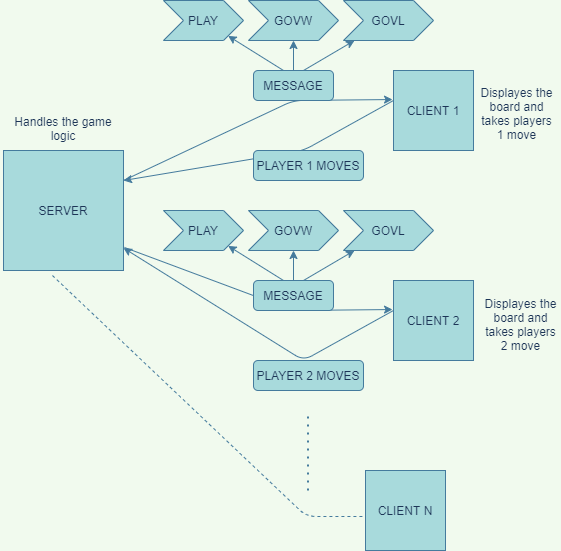
\includegraphics[width=\textwidth,height=\textheight,keepaspectratio]{appDiagram.png}
\end{figure}

\subsection{Application protocol}
The program waits for to clients to connect in order to start the playing session.\\\\
Once we have two players conneted the game starts in a recursive function called servicePlayers that stops when one of the players decides that he doesn't want to play anymore.\\\\
First it is checked if the game is over in which case we increment the score for the winner and we send the relevant messages for each client (the govw message to the winner and the govl message to the loser, both of them followed by score), then we aslo ask both players if they want a replay. If both of them asnwer affirmative then we call again the servicePlayer function, otherwise we close the connection to both clients and exit the servicePlayers function.\\\\
Then we start the actual game by sending the table to the first player and wait for the position that he wants to take (we do this for both players separately with a sleep() call between players), also we update the game board wiht the position that the player desires. 

\subsection{Server}
The server must start running before any client, and goes into an infinite loop to wait for clients\\ \\
When the server gets a client, it waits for another client (two players are needed)\\ \\
When the server gets the other client (now two clients), it forks and, let the child process take care of these two clients (players) in a separate function, called servicePlayers, while the parent process goes back to wait for the next two clients (players). Note that the file descriptors of the two connected sockets (one for each client) are passed to the function servicePlayers. \\ \\
The server handles the game logic and the score of both players for each session in the servicePlayers function.

\subsection{Client}

The clients establish the connection with the server and then waits in a infinite loop (that ends when the game over signal it is received) for messages from the server.\\
\\
The main purpose of the client is to display the board to the player and to take the next move of the player. All the positions that the players what to make would be validated directly in the client before sending them to the server.\\
\\
The client waits for 3 kind of messages from the server:\\
\begin{enumerate}
    \item The play message.
    \item The govw message (game over you won).
    \item The govl message (game over you lost)
\end{enumerate}
\\
\\
Each meesage triggers different reaction in the client respectively with the game logic.\\ \\
1) When we recieve the play message follow the steps:\\
\begin{itemize}
    \item We read the game board from the server. 
    \item Then we display the table to the player.
    \item We ask the player for the collum that he wants to move in.
    \item We transale the collum to the actual possition in the 2D array and then we send it to the server
\end{itemize}
\\ \\ 
2) When we recieve the govw message:
\begin{itemize}
    \item We tell the player that he won.
    \item We read the score board form the server and we display it to the player.
    \item We ask the player if he want to replay and send the answer back to the server.
\end{itemize}
3) When we recieve the govl messgae we follow the same steps as in hte govw but this time we say to the player that he lost.





\section{Implementation details}
\subsection{Server}
\clearpage
\begin{figure}[h!]
    \centering
    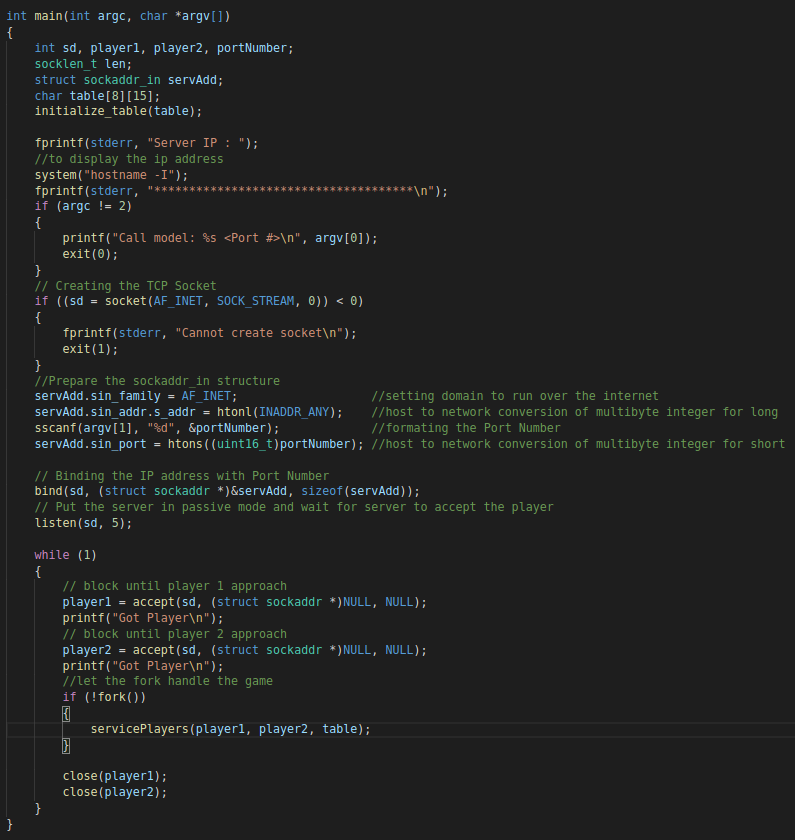
\includegraphics[width=1.3\textwidth,height=\textheight,keepaspectratio]{server_code.png}
\end{figure}


In the first part we prepare the data structures that we are going to use for the server, client and for the game itself.
We initialize the play board to be empty by calling the initialize\_table() function
\\Then we bind the server socket with the ip and the port values
\\We put the socket to listen to incoming clients
\\In a infinite loop we will do two consecutive accepts that will be blocking until we will have both players connected to the server
\\After we obtain the players each one with it's one descriptor we fork and let the child process handle the game session
\\In the forked process we call the servicePlayers function that takes as arguments the file descriptors for the clients and the game board and the scores for both players. This function  handles all the game logic
\subsection{Client}
\begin{figure}[h!]
    \centering
    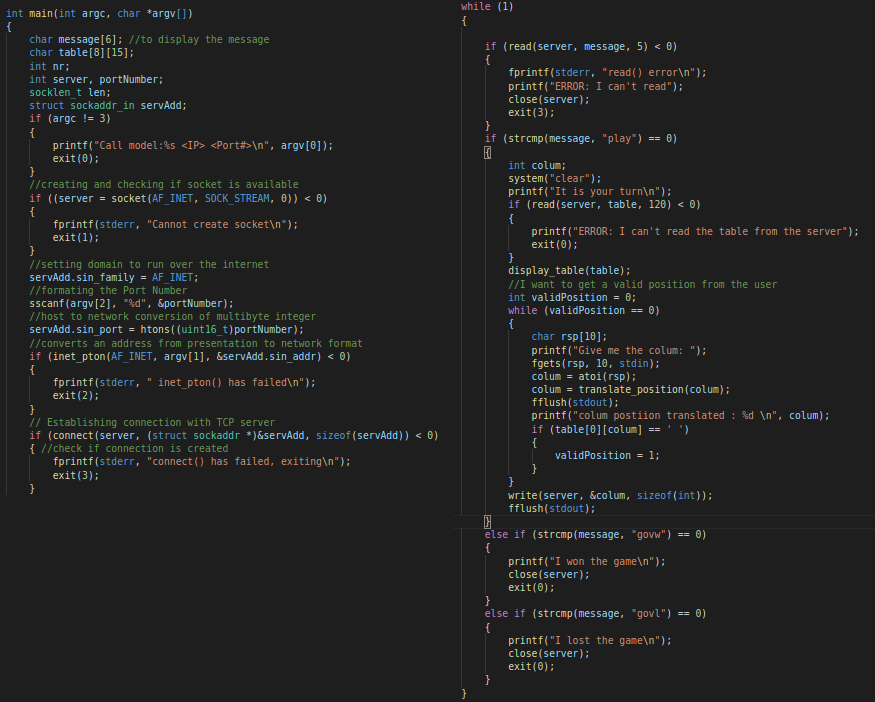
\includegraphics[width=1.3\textwidth,height=\textheight,keepaspectratio]{client_code.png}
\end{figure}
In the first part we establish the connection with the server\\
Then we enter a infinite loop in which we wait for different messages from the server
\\Case 1: we get the play message
\\We wait for the board then we ask the player for the next move, we check if the entered move is available (that collum most not be full already), we send the move to the server
\\Case 2: we get the govw message
\\govw message means that we won the game so we let the player know that he won and break the infinite loop and the connection with the server (in the future there will be a option to replay)
\\Case 3: we get the govl message
\\govl message means that the player lost the game, the steps are identical as in the case 2.

\begin{thebibliography}{9}
\bibitem{computer netwroks page}
  Computer Netwrorks Course page UAIC computer science faculty\\
  \url{https://profs.info.uaic.ro/~computernetworks/index.php}

\bibitem{Beej's Guide to Unix IPC}
  Beej's Guide to Unix IPC\\
  \url{http://beej.us/guide/bgipc/html/multi/index.html}
  
\bibitem{Beej's Guide to Network Programming}
  Beej's Guide to Network Programming\\
  \url{https://beej.us/guide/bgnet/html//index.html}
  
\bibitem{Beej's Guide to Network Programming}
  System programing - networking\\
  \url{https://github.com/angrave/SystemProgramming/wiki#8-networking}

\bibitem{Connect Four game}
  Connect four game\\
  \url{https://en.wikipedia.org/wiki/Connect_Four}  

\bibitem{Zombie procces prevemtion}
  Zombie processes prevention\\
  \url{https://www.geeksforgeeks.org/zombie-processes-prevention/}  
  
\end{thebibliography}  



\end{document}
